\section{Studies of jet properties}
\label{sec:jets}

First let us consider several variables that represent jet substructure using different types
of calorimeter granularity. The question we want to answer is how close the reconstructed
jet substructure variables reflect the input ``truth'' values  that are reconstructed using 
input particles directly from the \pythia generator.

In this study we use the jet effective radius and jet splitting scales as benchmark variables
to study jet substructure properties for different calorimeter granularity scenarios. 
The effective radius is the average of the energy weighted radial distance $\delta R_i$ in $\eta-\phi$ space of jet constituents.
It is defined as $(1/E) \sum_i e_i \delta R_i$, where $E$ is the energy of the jet and $e_i$ is the energy of a calorimeter 
cluster $i$ at the distance $\delta R_i$ from the jet center. The sum runs over all constituents of the jet. 
Recently, it has been studied for multi-TeV jets in Ref.\cite{Auerbach:2014xua}.
A jet $k_T$ splitting scale \cite{Butterworth:2002tt} is defined as a distance measure
used to form jets by the $k_T$ recombination
algorithm \cite{Catani1993187,Ellis:1993tq}.
This variable has been studied by ATLAS~\cite{ATLAS:2012am}, and more recently in the context of 100 TeV physics \cite{Auerbach:2014xua}.
The splitting scale is defined as 
$\sqrt{d_{12}}=\min(p_T^1,p_T^2) \times \delta R_{12}$ \cite{ATLAS:2012am} at the final stage of the $k_T$ clustering, where two subjets are merged into the final one.

Figures~\ref{fig:eff_rad} and  \ref{fig:d12} show the distributions of 
the jet effective radius and jet splitting scale for  different jet transverse momenta and HCAL granularities. 
The reconstructed-level distributions significantly disagree with the distributions  
reconstructed using truth-level particles. The distribution reconstructed with the cell
sizes 1~$\times$1~cm$^2$ are closest to the truth-level variables. The distributions 
reconstructed using the cell size of 20~$\times$20~cm$^2$, 
show the largest discrepancy with the
truth-level variables. Note that, in terms of closeness of reconstructed distributions to the truth level, 
there is no significant difference between 5~$\times$5~cm$^2$,  2~$\times$2~cm$^2$ and  1~$\times$1~cm$^2$ choices. 

Thus this study confirms the  baseline SiFCC detector geometry \cite{Chekanov:2016ppq}
that uses 5~$\times$~5~cm$^2$ cells,
corresponding to $\Delta \eta \times \Delta \phi = 0.022\times0.022$,
Note that the ATLAS and CMS detectors use the HCAL cell sizes in the barrel region which are close to 
$\Delta \eta \times \Delta \phi = 0.1\times0.1$.  According to this study,
such HCAL cell sizes are not optimal in terms of performance  for tens-of-TeV jets.

In the next few sections we will consider several other physics-motivated
variables that can shed light  upon the performance of the HCAL for tens-of-TeV jets.

\begin{figure}
\begin{center}
   \subfigure[5 TeV] {
   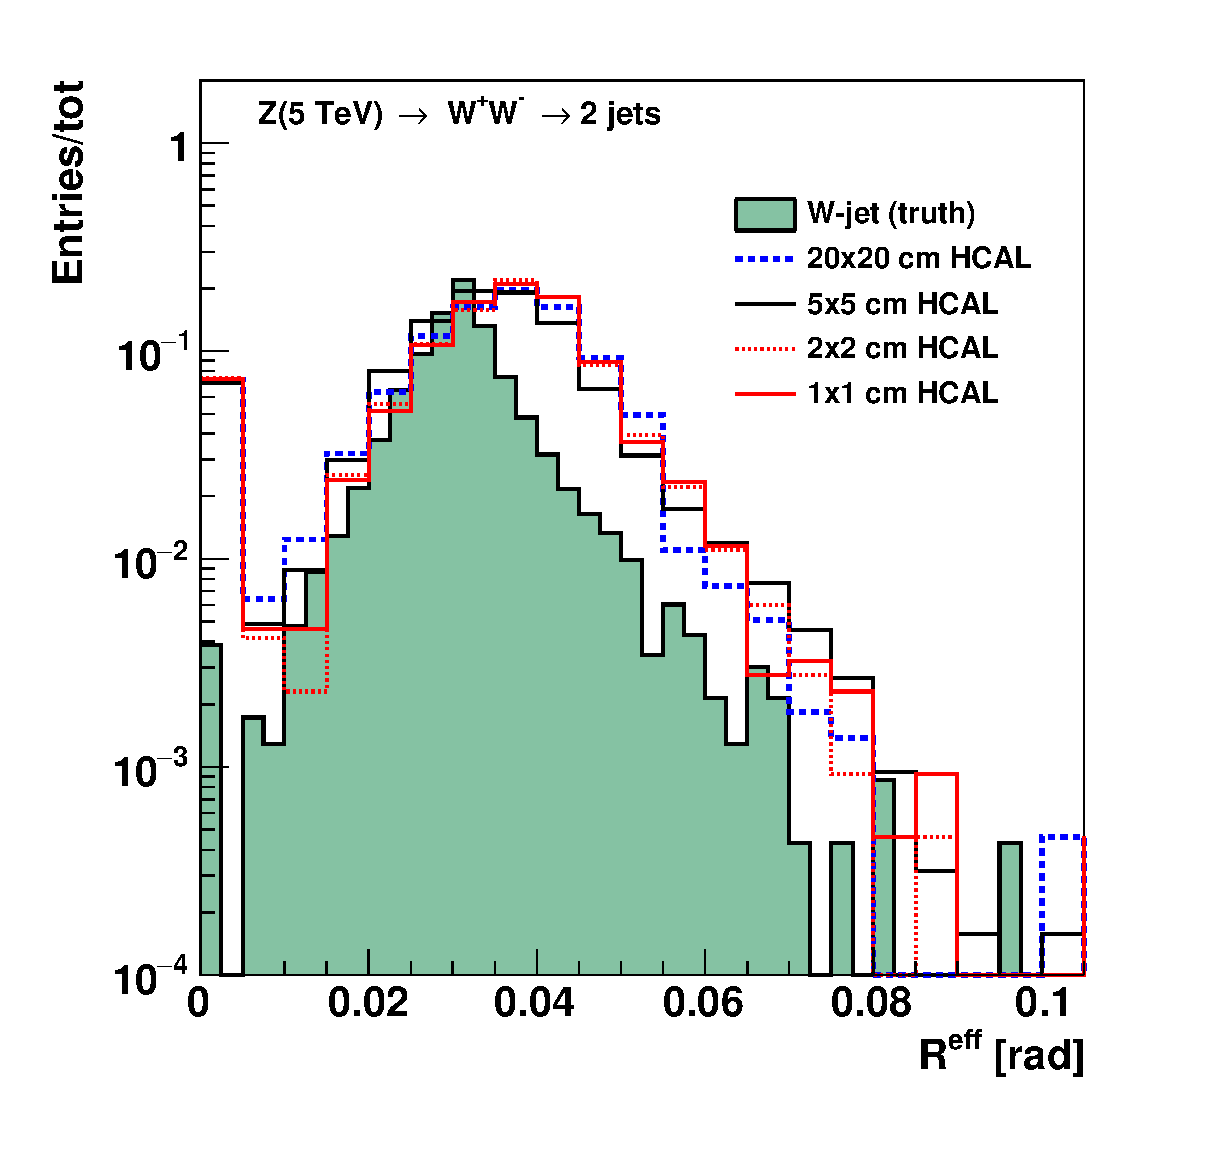
\includegraphics[width=0.46\textwidth]{figs/h5tev_clus_effR_ww1}\hfill
   }
   \subfigure[10 TeV] {
   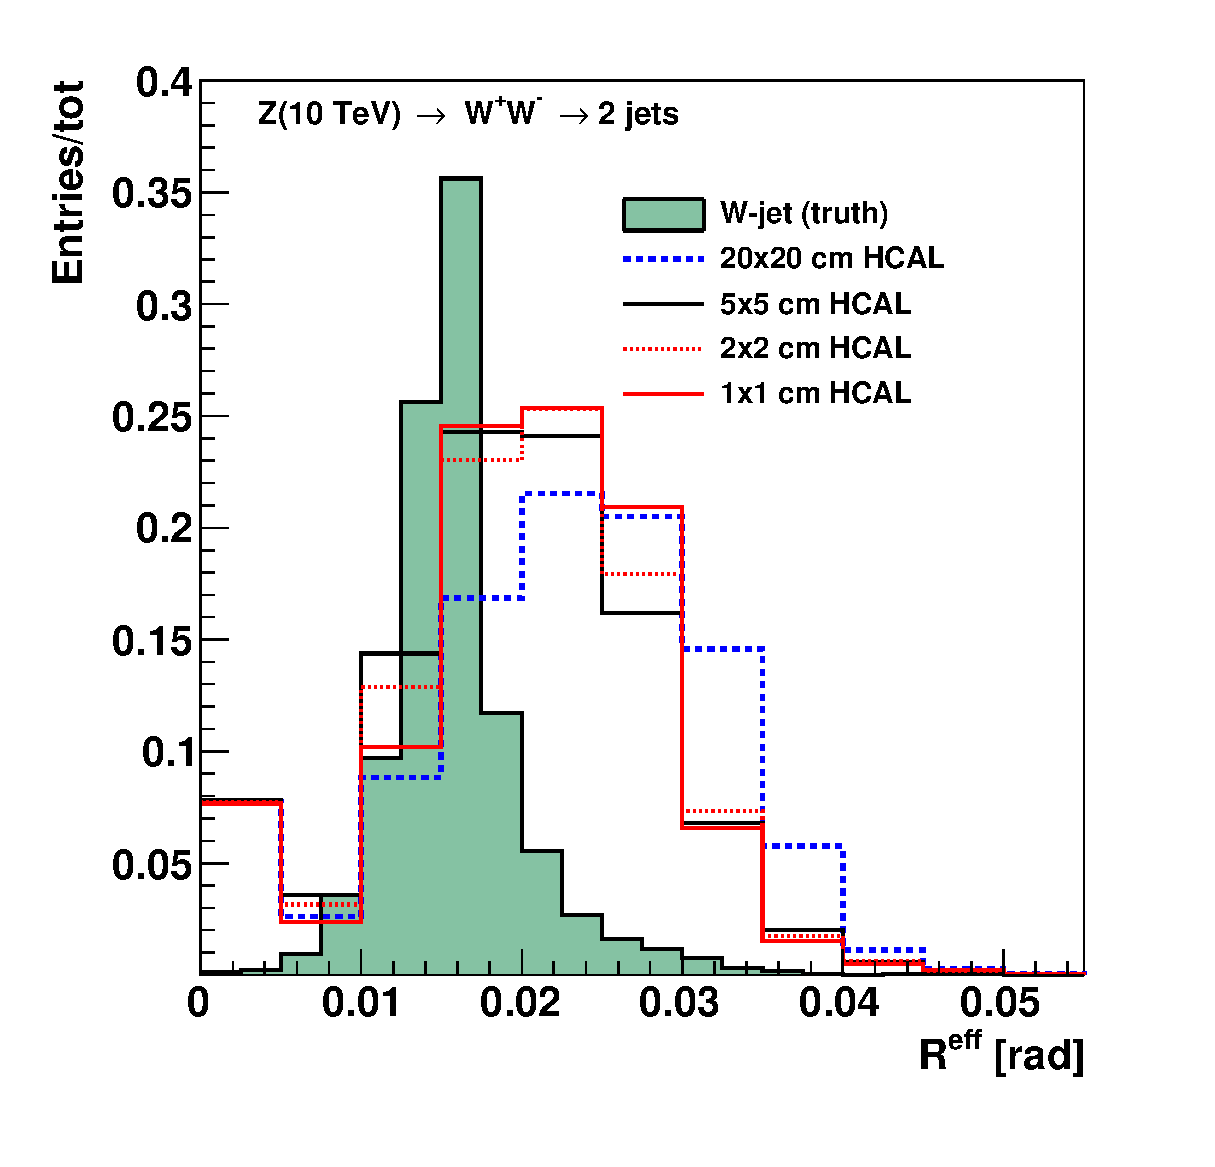
\includegraphics[width=0.46\textwidth]{figs/h10tev_clus_effR_ww1}
   }
   \subfigure[20 TeV] {
   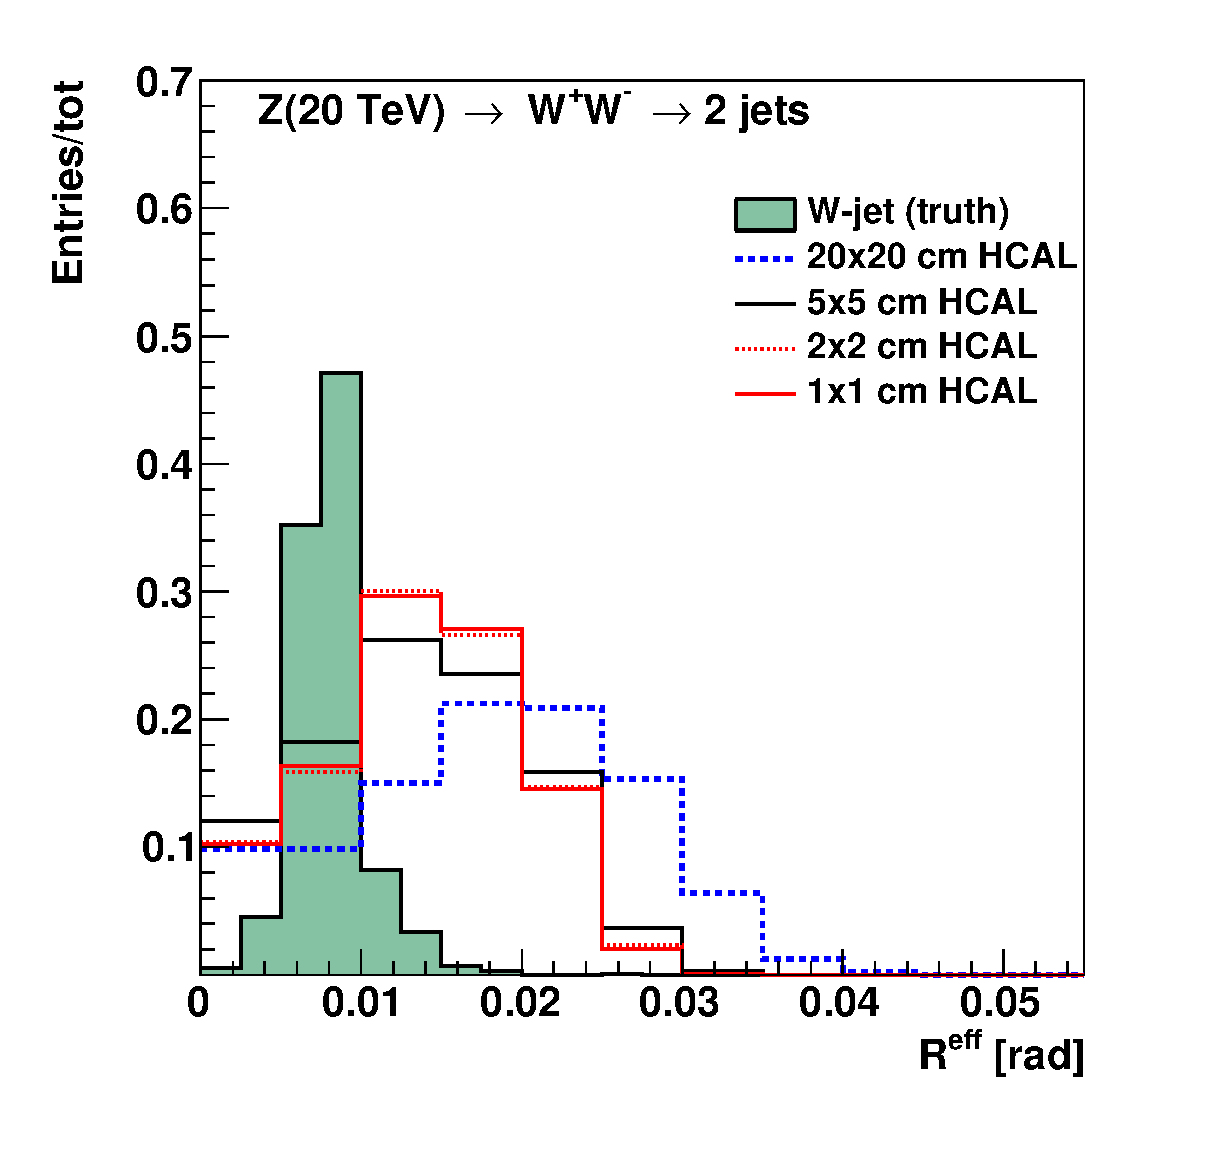
\includegraphics[width=0.46\textwidth]{figs/h20tev_clus_effR_ww1}
   }
   \subfigure[40 TeV] {
   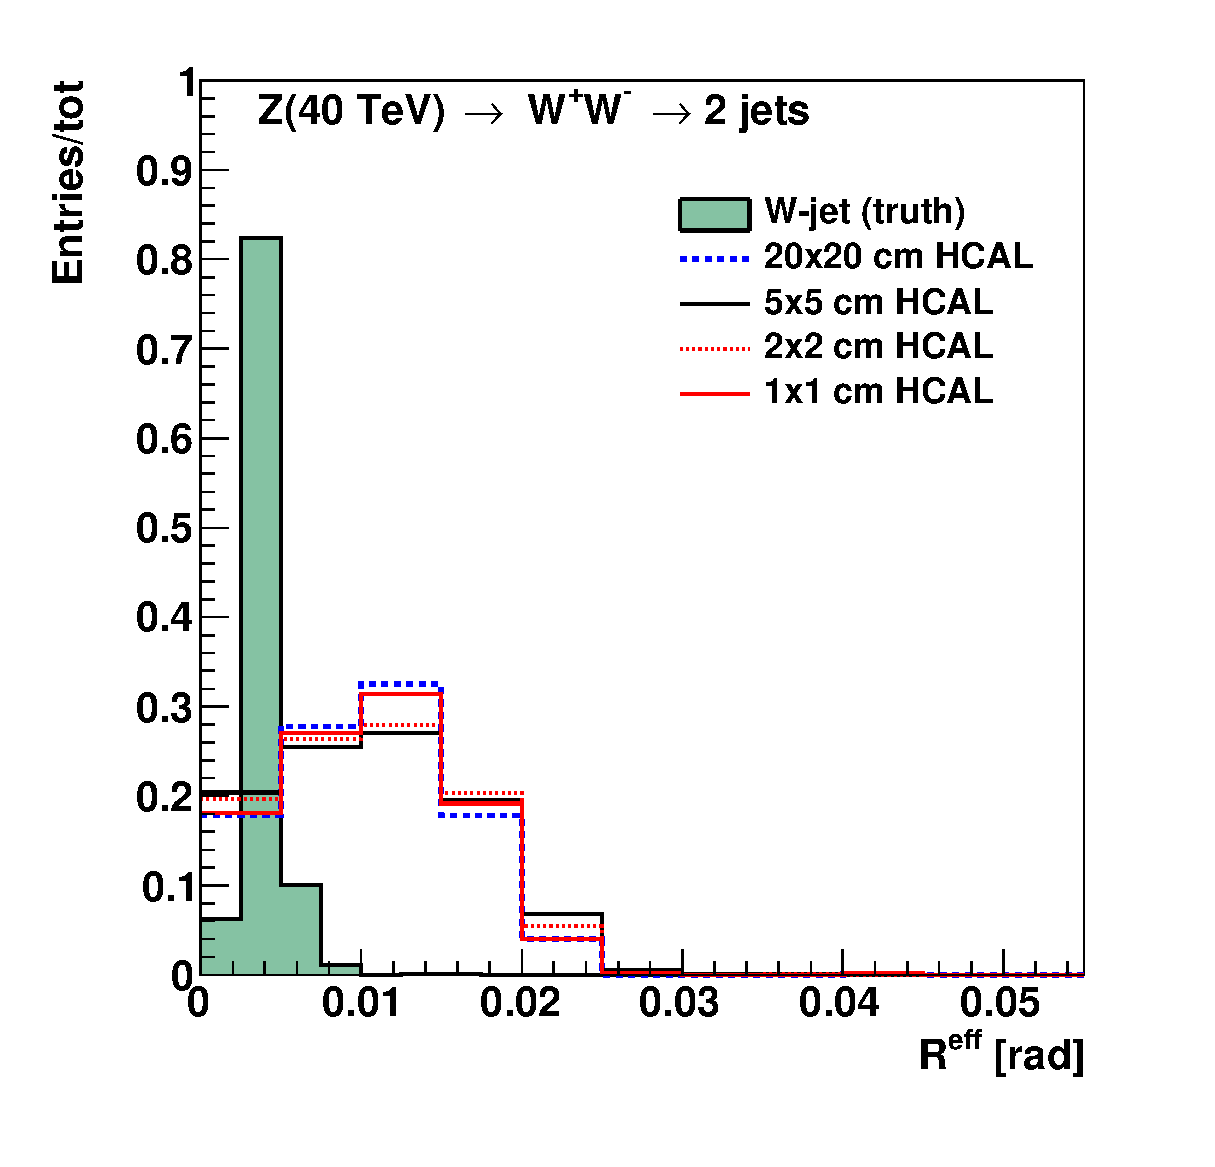
\includegraphics[width=0.46\textwidth]{figs/h40tev_clus_effR_ww1}
   }
\end{center}
\caption{Jet effective radius for different jet transverse momenta and HCAL granularities.}
\label{fig:eff_rad}
\end{figure}


\begin{figure}
\begin{center}
   \subfigure[5 TeV] {
   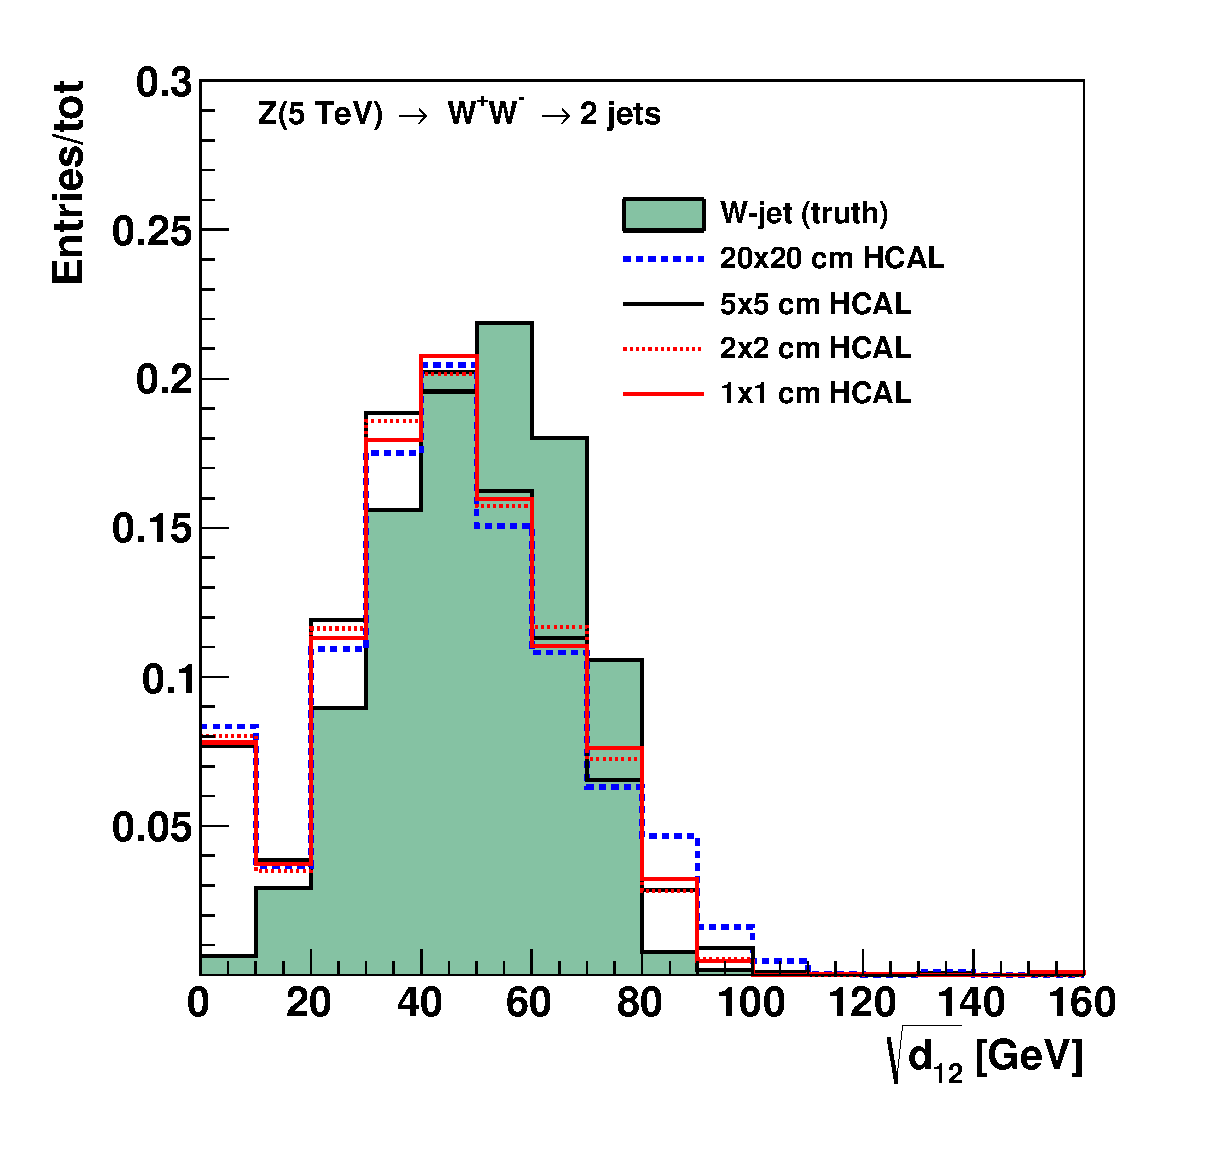
\includegraphics[width=0.46\textwidth]{figs/h5tev_clus_d12_ww1}\hfill
   }
   \subfigure[10 TeV] {
   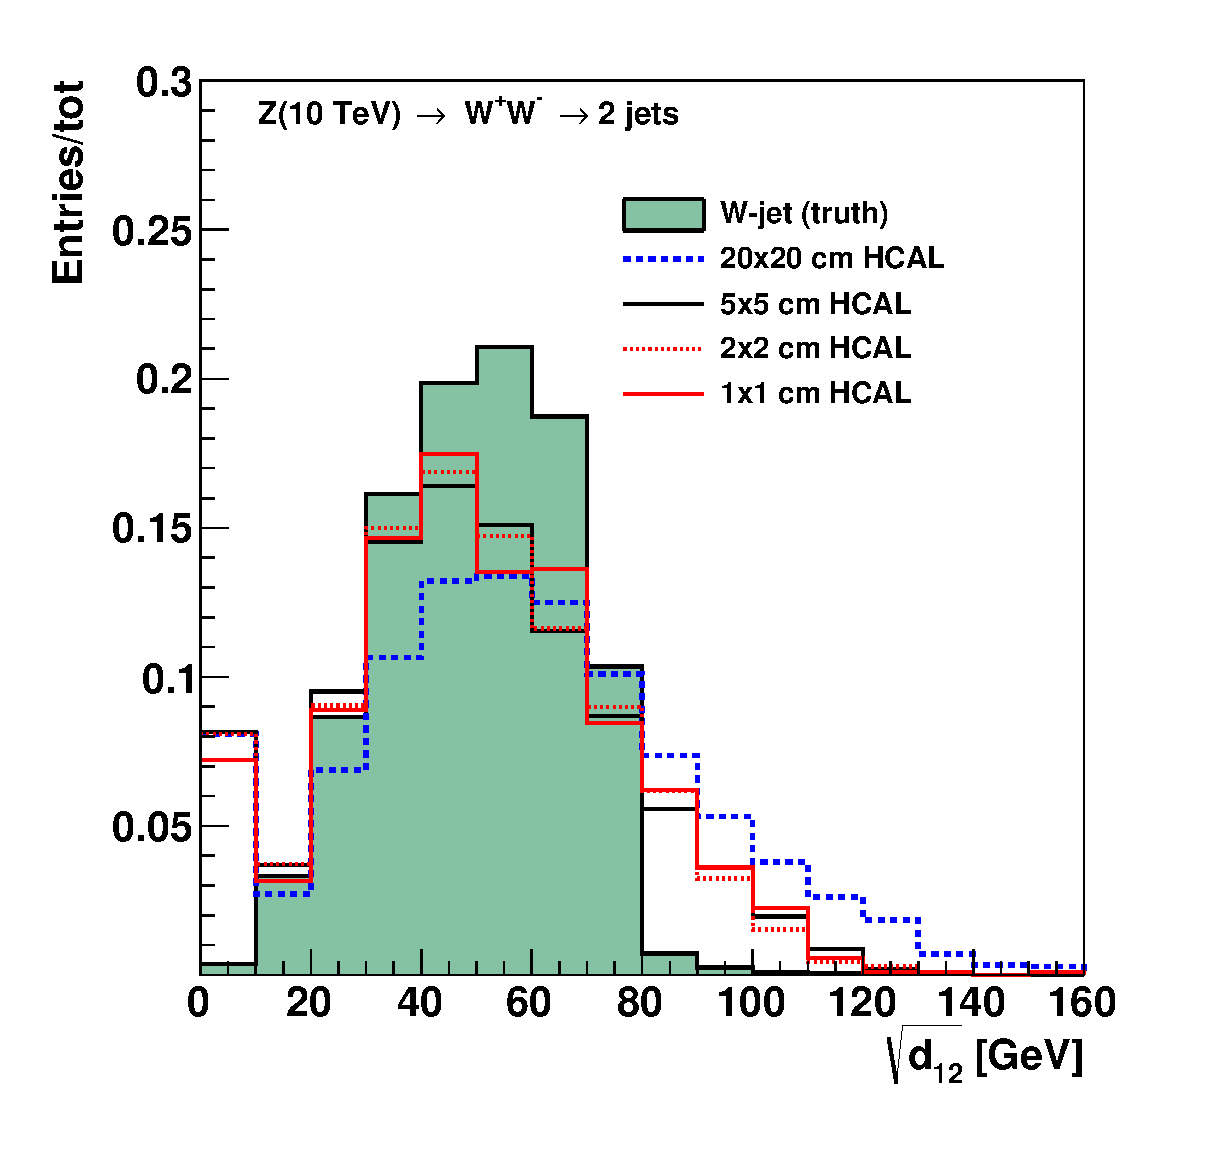
\includegraphics[width=0.46\textwidth]{figs/h10tev_clus_d12_ww1}
   }
   \subfigure[20 TeV] {
   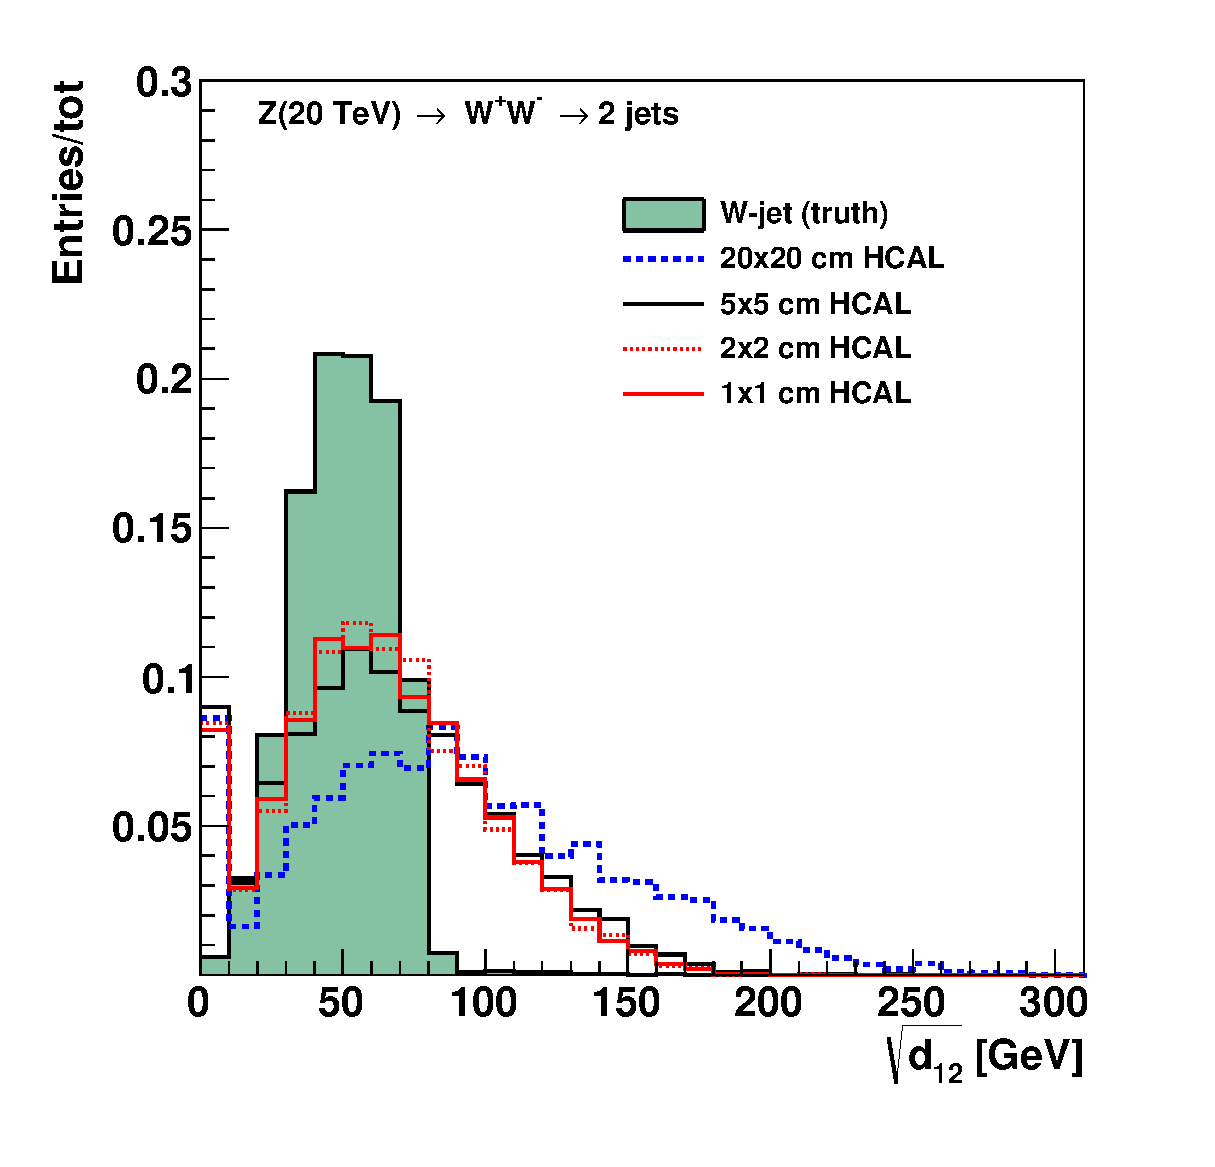
\includegraphics[width=0.46\textwidth]{figs/h20tev_clus_d12_ww1}
   }
   \subfigure[40 TeV] {
   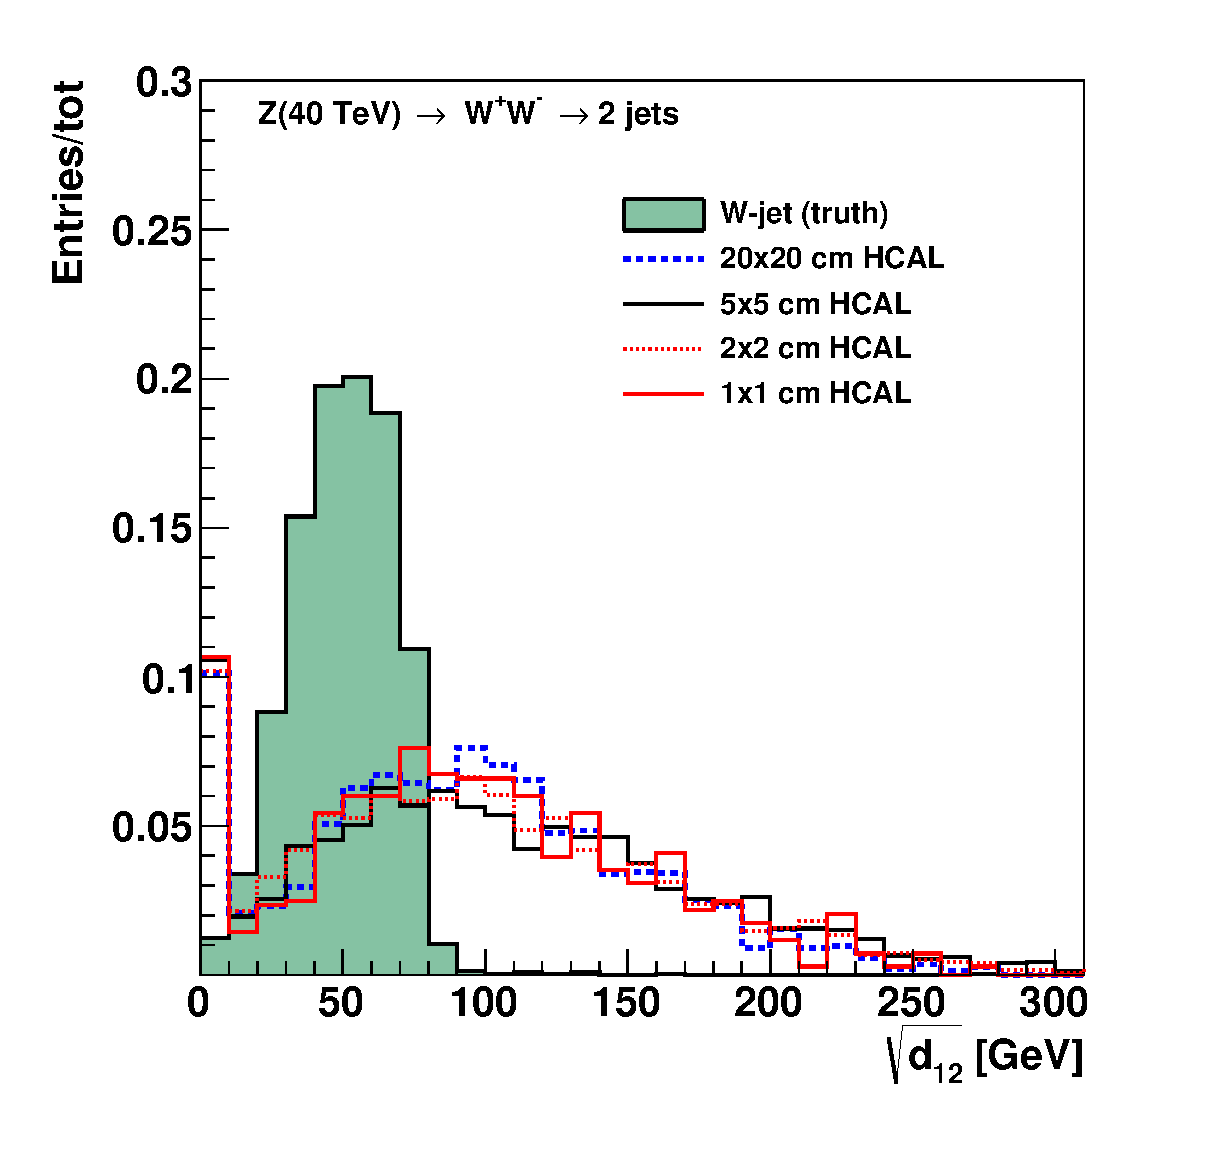
\includegraphics[width=0.46\textwidth]{figs/h40tev_clus_d12_ww1}
   }
\end{center}
\caption{Jet splitting scale for different jet transverse momenta and HCAL granularity.}
\label{fig:d12}
\end{figure}


%%%%%%%%%%%%%%% commented out 
\begin{comment}

\subsection{Jet subjettiness}

We recall that $N$-subjettiness~\cite{Thaler:2010tr}, $\tau_{N}$, of jets has been proposed
as a class of variables with which to study the decay products of a heavy particle inside jets.  $\tau_{N}$ is a measure of the degree to which a jet can be considered as being composed of
 $N$  $k_{T}$-subjets \cite{Thaler:2010tr}. 
The variable $\tau_{32}$, defined as the ratio of the $N$-subjettiness variables $\tau_3/\tau_2$, is particularly sensitive to hadronically-decaying
 top-quark initiated jets.
The variable, $\tau_{21} \equiv \tau_2/\tau_1$ can be used to reject background from $W/Z$ decays.
These variables do not strongly correlate with jet mass and can provide an independent check for the
presence of top quarks.
The jet substructure variables were obtained by re-running the $k_T$ algorithm over the jet constituents of anti-$k_T$ jets.

As an example of the effect of the calorimeter granularity, 
\begin{figure}
\begin{center}
   \subfigure[5 TeV] {
   \includegraphics[width=0.43\textwidth]{figs/r09_tau21b1_20tev_04_U.pdf}\hfill
   }
   \subfigure[10 TeV] {
   \includegraphics[width=0.43\textwidth]{figs/r010_tau21b1_20tev_04_U.pdf}
   }
   \subfigure[20 TeV] {
   \includegraphics[width=0.43\textwidth]{figs/r012_tau21b1_20tev_04_U.pdf}
   }
\end{center}
\caption{Jet subjetinness $\tau_{21}$ for jets originating from splitting scale for different jet transverse moment and HCAL granularity.}
\label{fig:tau21}
\end{figure}


\begin{figure}
\begin{center}
   \subfigure[5 TeV] {
   \includegraphics[width=0.43\textwidth]{figs/r09_tau32b1_20tev_04_U.pdf}\hfill
   }
   \subfigure[10 TeV] {
   \includegraphics[width=0.43\textwidth]{figs/r010_tau32b1_20tev_04_U.pdf}
   }
   \subfigure[20 TeV] {
   \includegraphics[width=0.43\textwidth]{figs/r012_tau32b1_20tev_04_U.pdf}
   }
\end{center}
\caption{Jet subjetinness $\tau_{32}$ for jets originating from splitting scale for different jet transverse moment and HCAL granularity.}
\label{fig:tau21}
\end{figure}

%%%%%%%%%%%%%%% commented out 
\end{comment}

